% !TEX root = ../../report.tex

\subsection{PCB Results (fixes)}

Due to the manual work involved in designing the PCB, and because it was fairly
unfamiliar ground for everyone involved, there were many things that could go
wrong. This section describes everything that was wrong with the PCB along with
what was done to fix it.

The first thing to happen was smoke appearing from the linear regulator upon
plugging in the power source. As it turned out, the footprint was mismatched
with the pinout of the component. The footprint had been fixed early on in the
process, but unfortunately the schematics had not been updated. The same turned
out to have happened with the low frequency crystal connected to the MCU,
although this component did not produce any smoke.

Both of the above problems where solved by extra wiring. For the crystal, where
pin 1 and 4 was suppose to be used, pin 1 and 2 were used instead. As pins 2 and
3 were unconnected, a patch cable was soldered between pin 4 and 2.
\missingfigure{picture with textual reference}

The linear regulator was slightly more advanced as pin 1 and 5, and 2, 3 and 4,
had been swapped. The solution was to solder six short patch cables on the pads
themselves, and then match the feet of the linear regulator with the right
cables. This resulted in the linear regulator being mounted about 1 cm above the
card.

\begin{figure}[H]
    \centering
    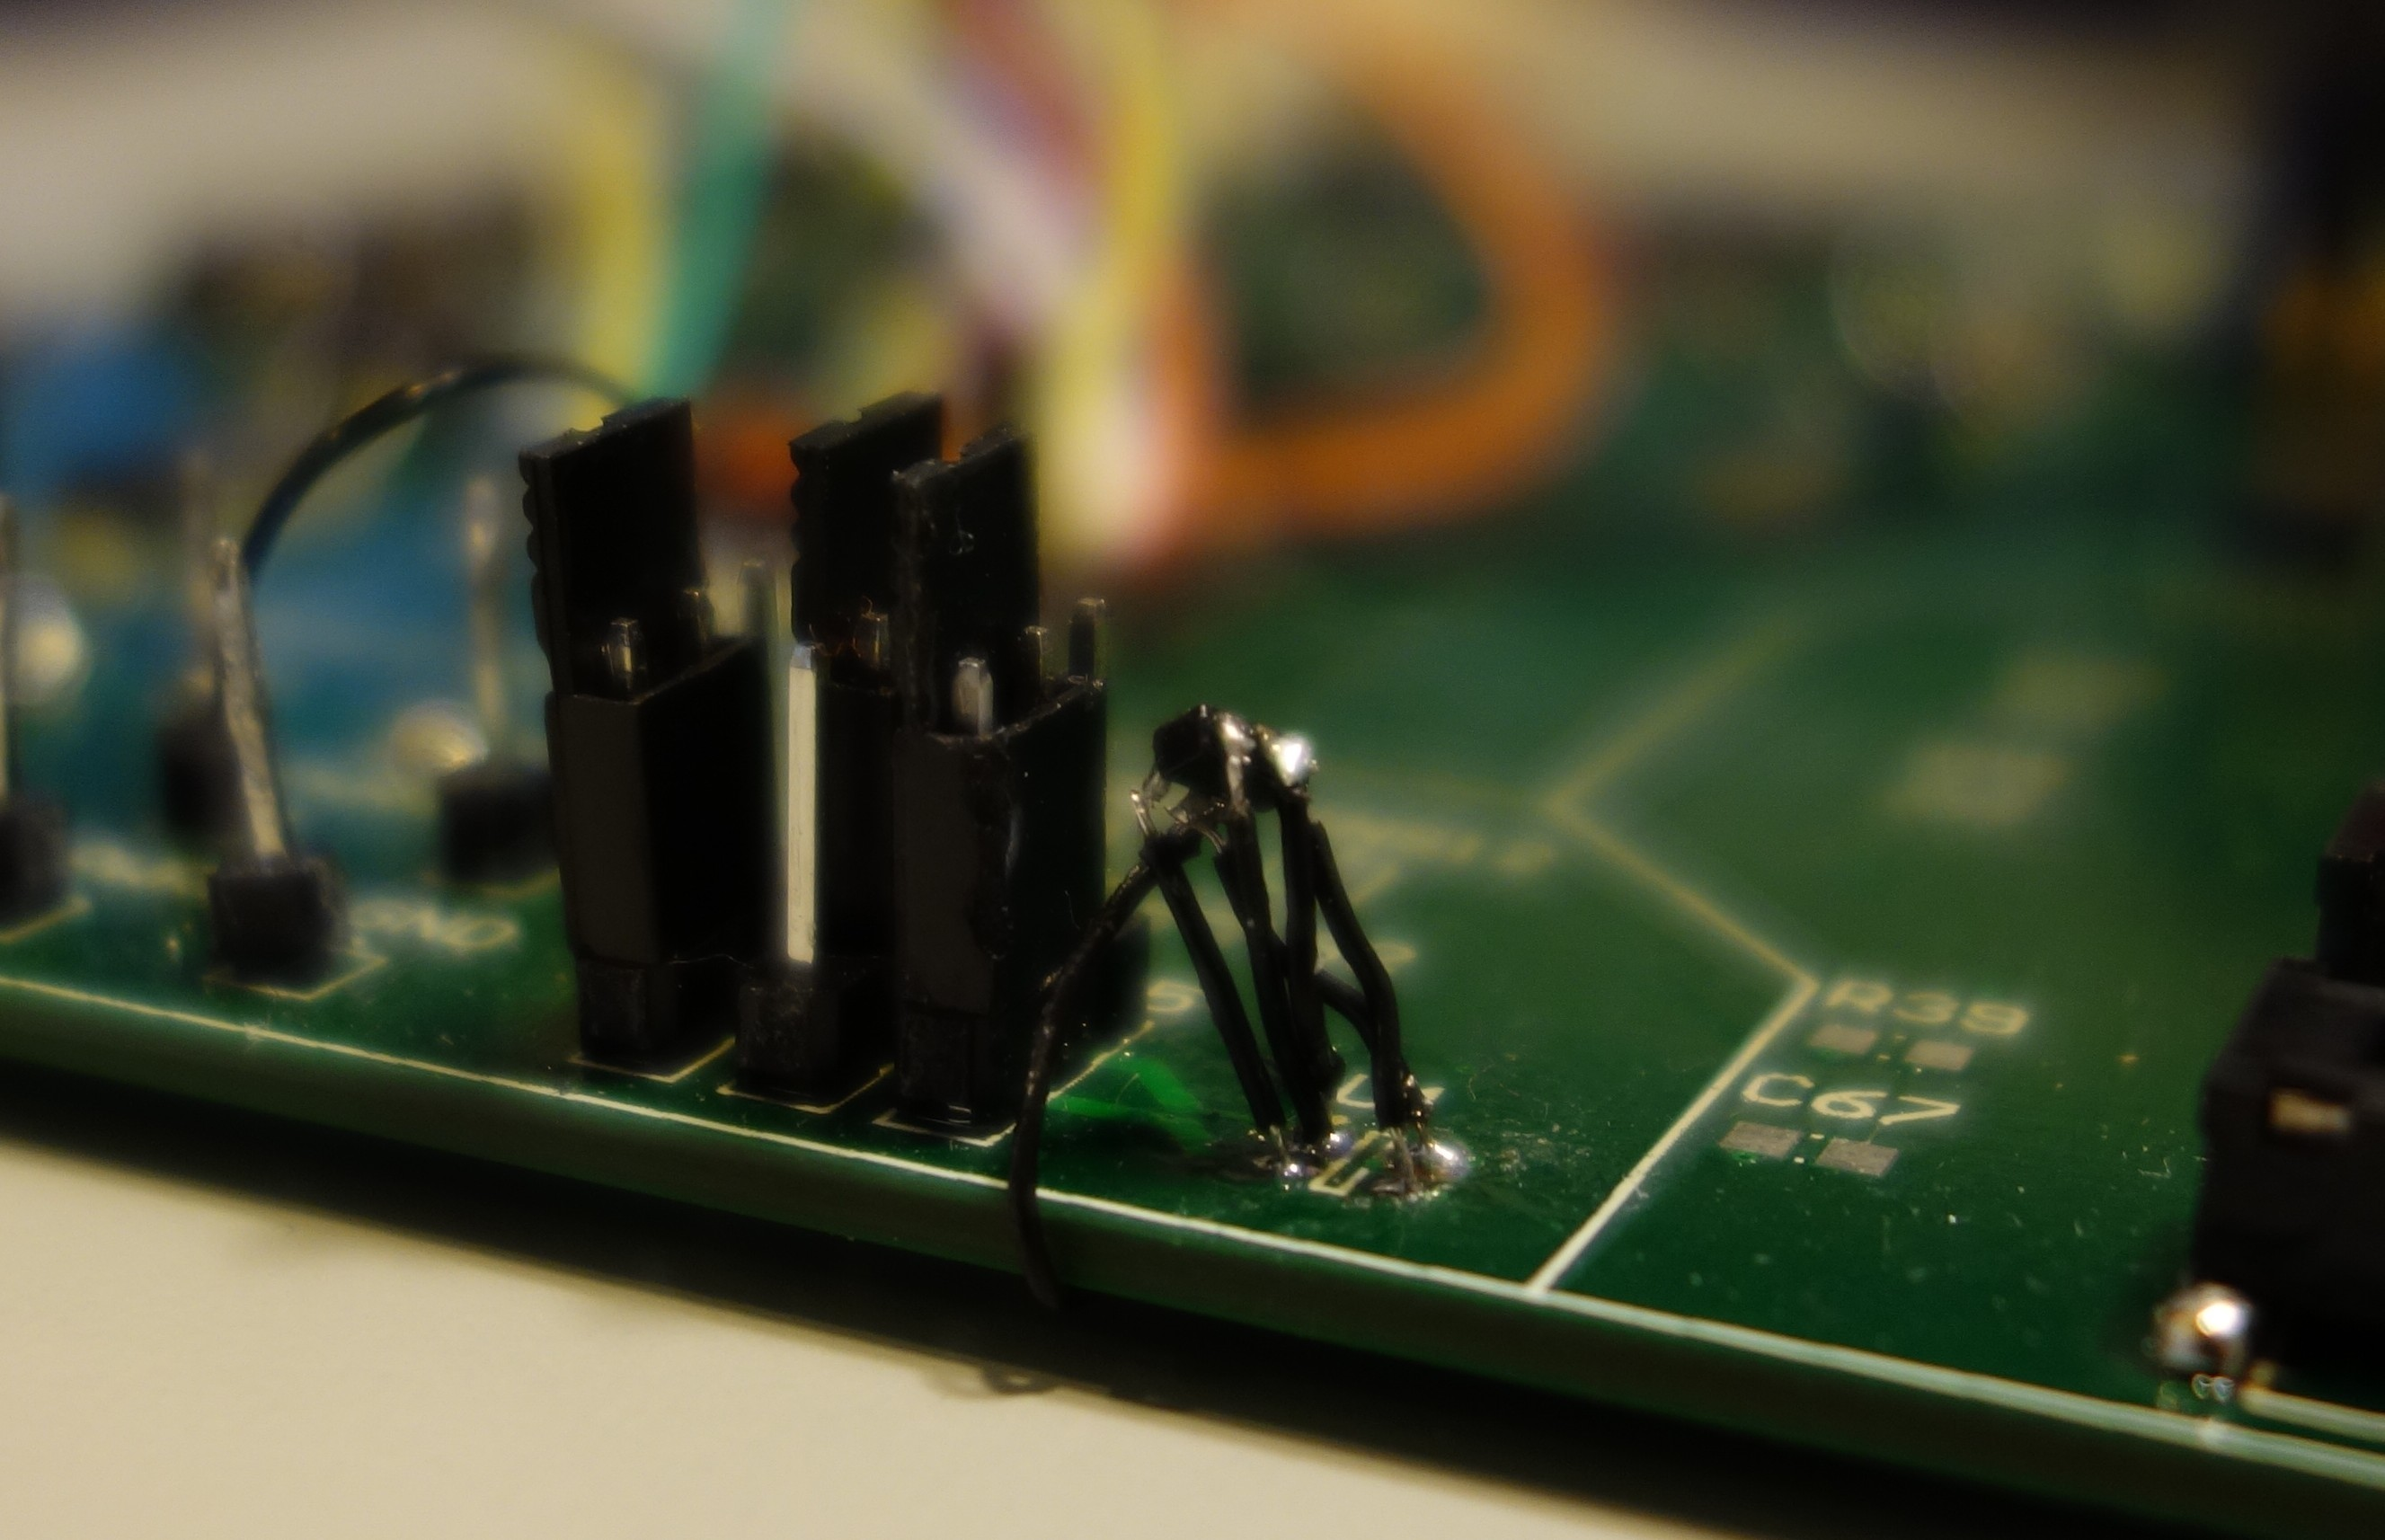
\includegraphics[scale=0.1]{figures/results/pcb/linear-regulator.jpg}
    \caption{Linear voltage regulator hack.}
    \label{fig:res:linreg}
\end{figure}



In addition, there was an actual connection error in the external RAM footprint.
One of the two chip select inputs, CS1, was suppose to be grounded, but had
mistakenly been connected to VCC33, resulting in the unit being stuck in off
mode. To solve this, the chip select pin was bent slightly upwards and then
connected with a patch cable to a GND pin nearby. \missingfigure{photo. Textual
reference.}

Finally, due to a typo in the schematic, the data lines of the EBI bus were only
connected to the MCU and external RAM, not to the FPGA. Again, this was solved
by patch cables between the external RAM's data pins and all available FPGA GPIO
pins. The result was a fully functional bus as was originally intended, at the
expense of all other I/O opportunities on the FPGA. All 12 GPIO pins were used,
as well as two buttons and two LED's, adding up to 16 bits.\missingfigure{photo
of the hack}
